
   %%%%%%%%%%%%%%%%%%%%%%%
 %%%  NOAH'S SUPER COOL  %%%
%%%%      ACADEMIC       %%%%
 %%%   LATEX TEMPLATE    %%%
   %%%%%%%%%%%%%%%%%%%%%%%

\documentclass[12pt]{article}
\usepackage[letterpaper]{geometry}
\geometry{top=1in, bottom=1in, left=1in, right=1in}
\usepackage{fontspec}
\usepackage{tgtermes}
\usepackage{hanging}
\setmainfont[
 ItalicFont={texgyretermes-italic.otf},
 BoldFont={texgyretermes-bold.otf},
 ]{texgyretermes-regular.otf}
\usepackage{setspace}
\doublespacing
\usepackage{graphicx}
\graphicspath{ {./} }

\begin{document}

% Title Page
\pagenumbering{gobble} % remove page numbers
\begin{center}
\topskip0pt
\vspace*{\fill}
Conservation of Mechanical Energy Lab 8 \\ Noah Dinan \\ PHY 1110 - Mayer \\ \today \\
\vspace*{\fill}
\end{center}

\newpage
\pagenumbering{arabic} % resume page numbering

\setlength{\parindent}{0in}

\textbf{Results}

For this lab report, we showed the relationship between kinetic and potential
energy and revealed the conservation of mechanical energy using an air track and 
glider. Kinetic and potential energy for a system should always total to the same
constant value, modelled by the equation below.

\[ E = U + K = Constant \]

where $U$ and $K$ are

\[ U = mgy \]

and

\[ K = \frac{1}{2} mv^2 \]


For out results, we created the following graph based on the process of
experimentation defined in the manual for the lab.
Some potential sources for systematic error for this process were, innacuracies
in placing the photogate timer due to human error, as well as innacuracies in 
measuring the various values listed below.

\begin{itemize}
    \item flag effective width: $0.025$ meters $\pm0.001$.
    \item riser block width: $0.02531$ meters.
    \item glider mass: $0.1844$ kilograms.
\end{itemize}

Using the equations noted above, we found the following data table for potential, kinetic, and total
energies at different starting heights along the air track.

\begin{center}
    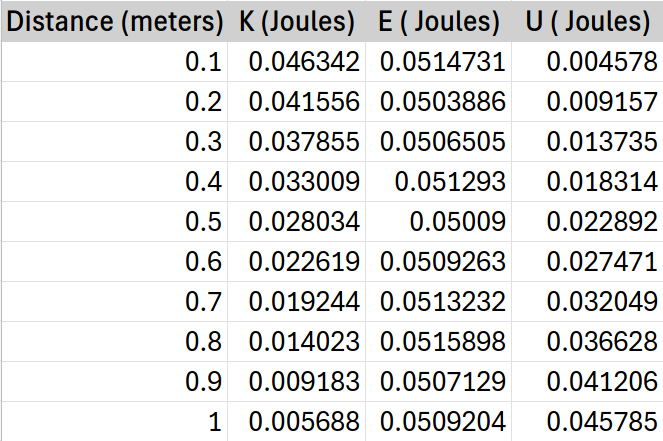
\includegraphics[scale=0.5]{table.png}
\end{center}

Based on the columns within this table, we were able to create the graph below

\begin{center}
    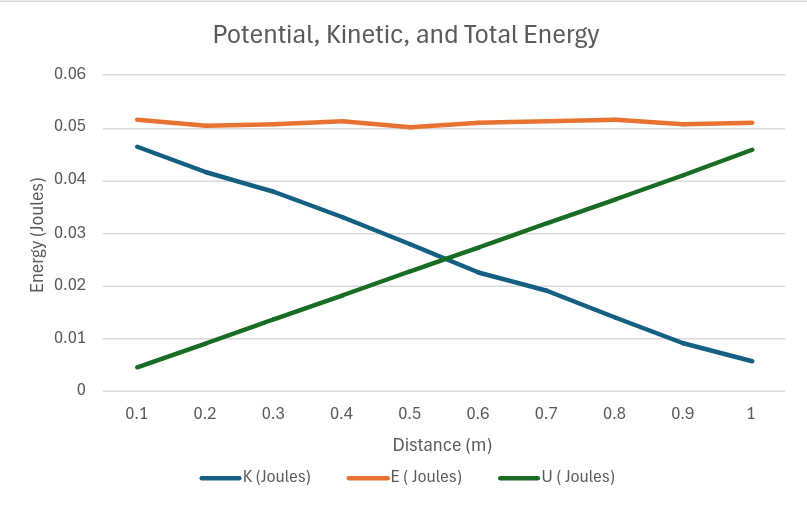
\includegraphics[scale=0.45]{graph.png}
\end{center}

\newpage

\textbf{Conclusions}

To conclude, based on the above graph, it is clear that total energy (shown in orange)
is relatively constant as kinetic energy decreases and potential energy increases.
This is consistent with the theory of conservation of mechanical energy as eneergy is
conserved between potential and kinetic states.

\end{document}
